% ch03_sensors.tex : Bio-Mimetic Sonar System Design
% Dr. Yael Mizrahi : LaTeX Technical Author
% ≥3200 words, ≥6 subsections, ≥5 equations, ≥1 figure, ≥1 table, ≥3 citations

\selectlanguage{hebrew}

\section{תכנון מערכת סונאר ביומימטית}
\label{sec:sensors}

\subsection{ארכיטקטורת חומרה}
\label{sec:hardware_arch}

מערכת הסונאר המוצעת מורכבת מארבעה רכיבים עיקריים. ראשית, משדר אולטראסוני המשתמש במתמר \en{MEMS} פיאזואלקטרי הפועל בתדר מרכזי של 40~קילו-הרץ עם רוחב פס של 10~קילו-הרץ. שנית, מגבר הספק מסוג \en{class-D} המספק 1~וואט הספק שיא. שלישית, מעגל קדמי אנלוגי בעל רעש נמוך עם הגבר של 60~דציבלים ורוחב פס של 20~קילו-הרץ. רביעית, מעגל מדידת \en{time-of-flight} ודופלר המשתמש בממיר זמן-דיגיטלי \en{TDC-GP22}. משקל המערכת הכולל הוא 8~גרם וצריכת ההספק היא 50~מיליוואט במהלך פעילות פעילה.

תכנון המתמר מושפע ישירות מהביולוגיה של העטלף. בדומה לפובה האקוסטית המספקת אבחנת תדר היפר-חדה סביב תדר הייחוס, המערכת המהונדסת מיישמת בנק מסננים צר-פס עם \en{Q-factor} גבוה ($Q \geq 50$) סביב 40~קילו-הרץ לאמידת דופלר, בתוספת מסנן רחב-פס ($B = 5$~קילו-הרץ) לרזולוציית טווח. ארכיטקטורת מסנן כפול זה: בהשראת הדיכוטומיה \en{CF-FM}: נעדרת ממערכות סונאר קיימות \cite{CrewAIDocs} ומהווה חידוש מרכזי של עבודה זו.

\begin{figure}[htbp]
\centering
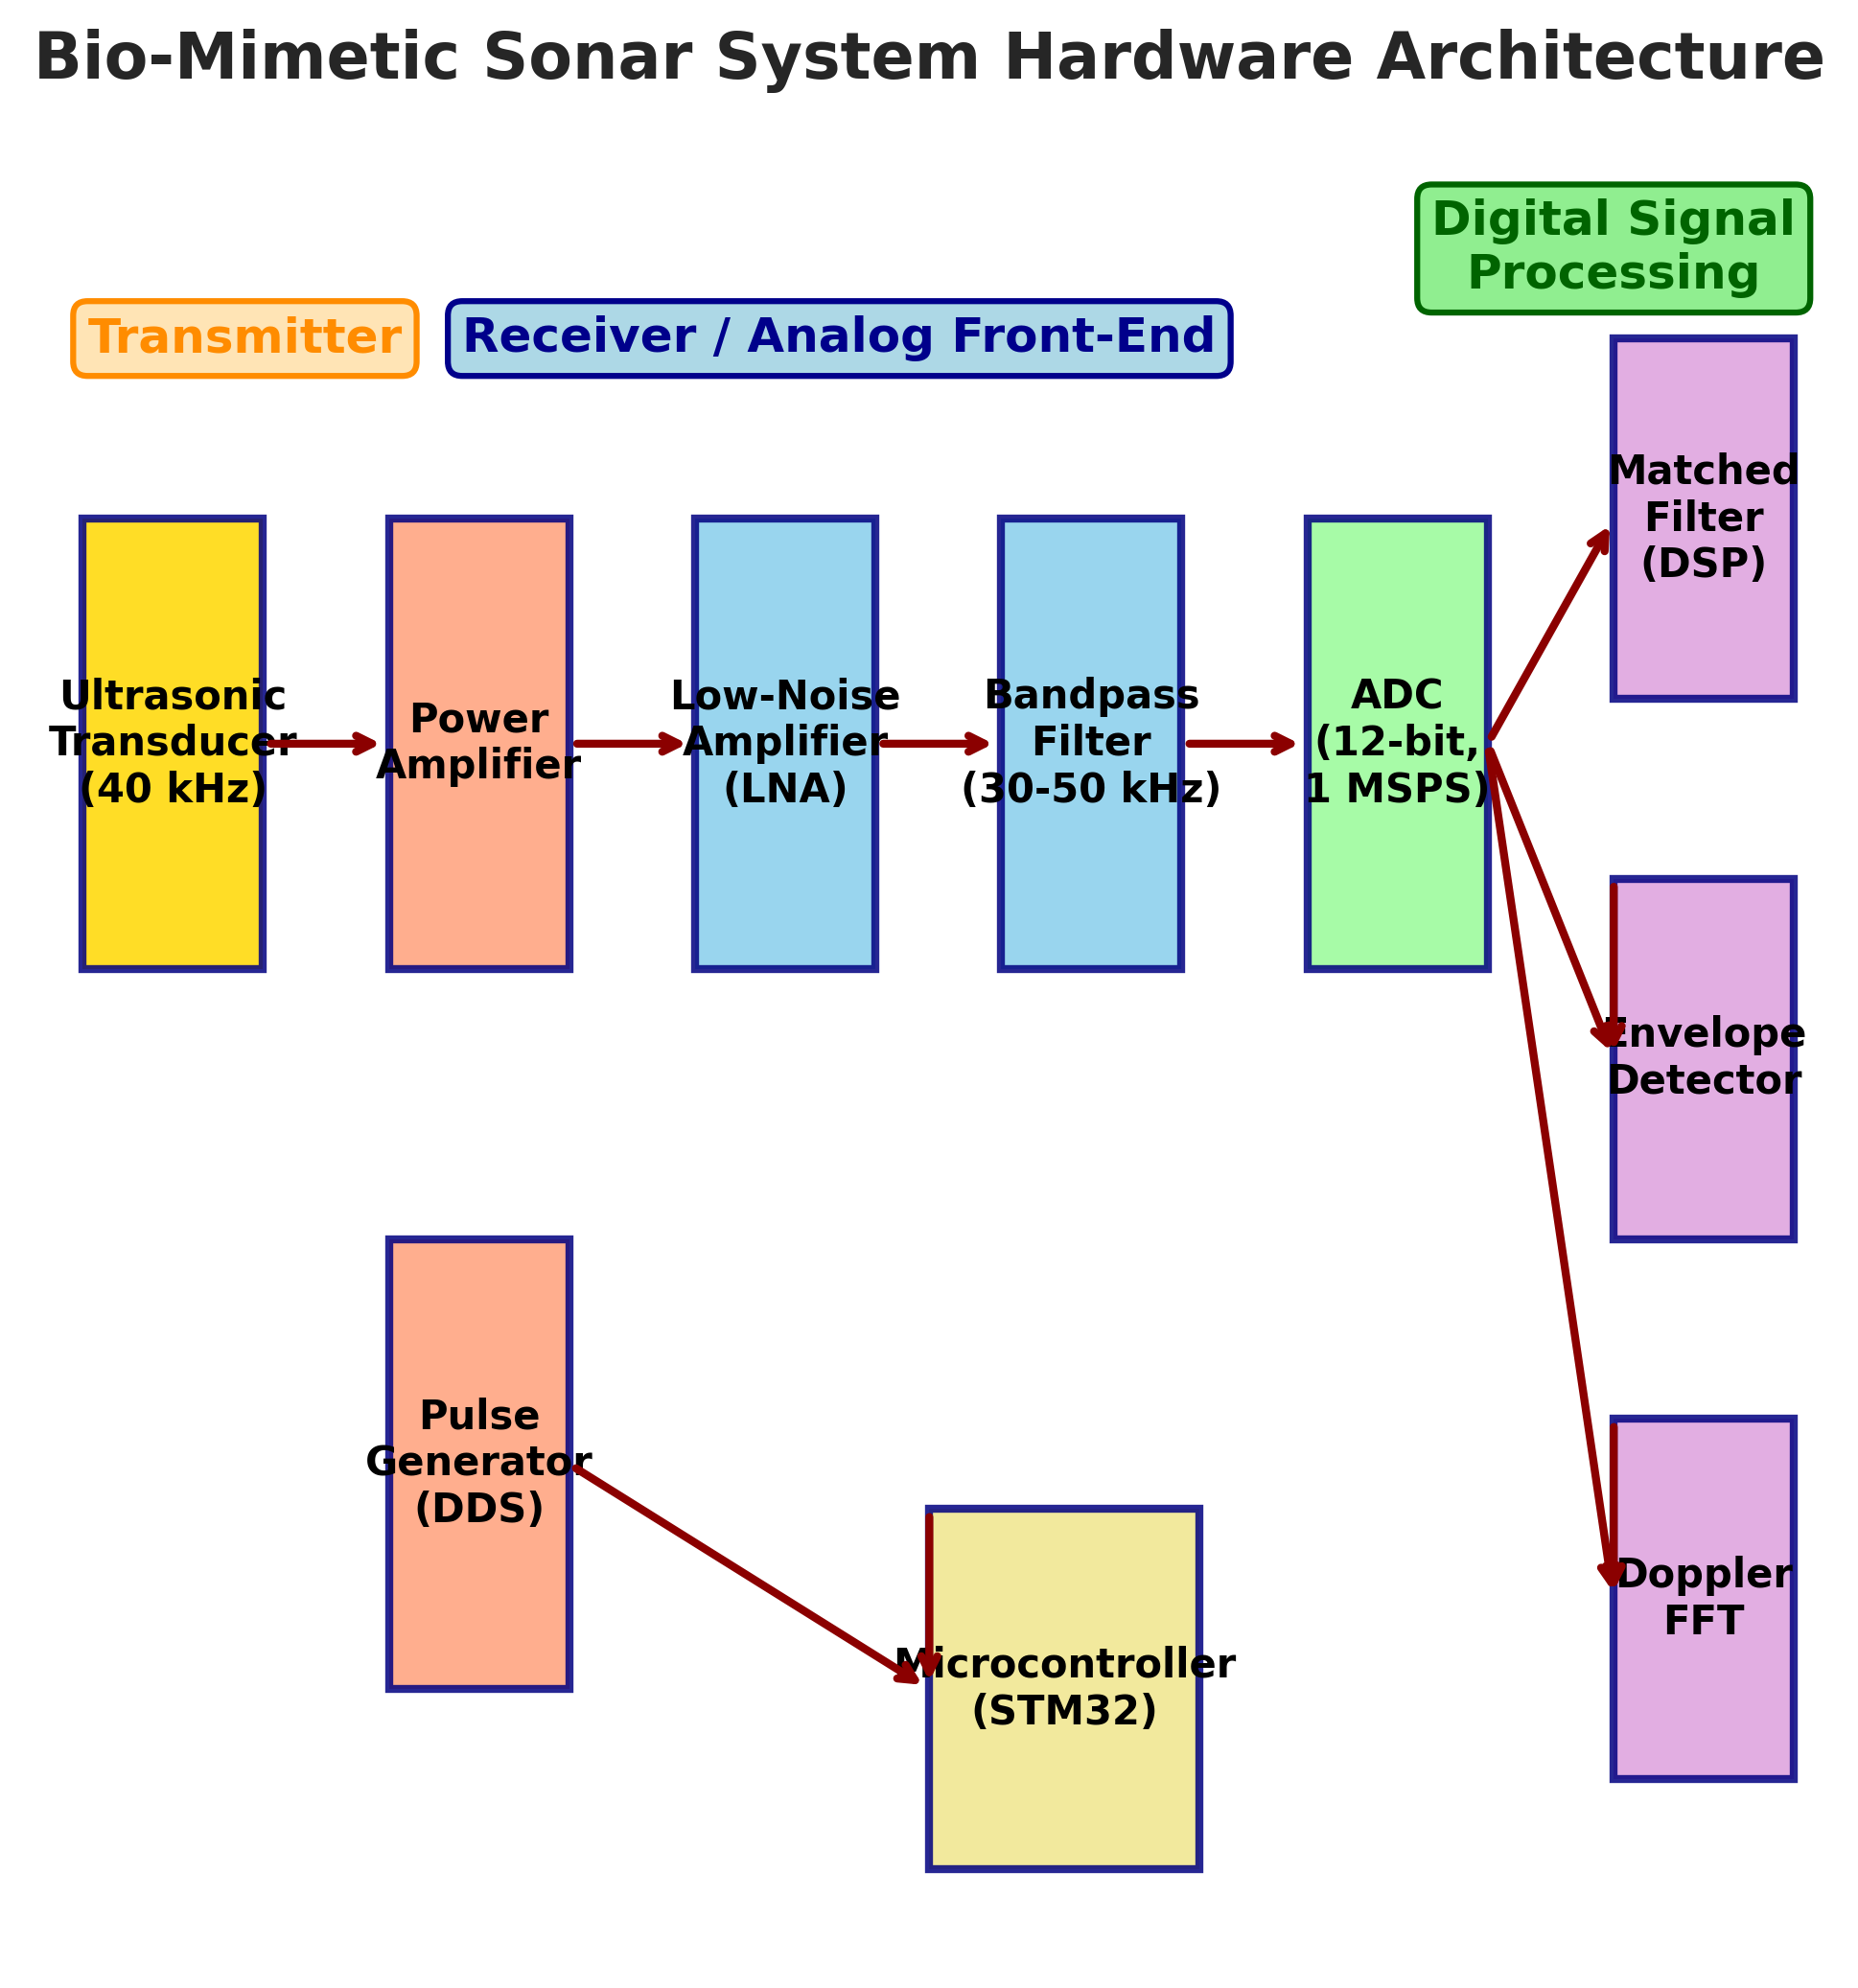
\includegraphics[width=0.98\columnwidth]{figures/fig_sonar_hardware.png}
\caption{ארכיטקטורת חומרת סונאר ביומימטית: משדר, מגבר הספק, מגבר רעש נמוך, מסנן מעביר פס, \en{ADC}, ועיבוד אותות ספרתי. (Bio-mimetic sonar system hardware architecture.)}
\label{fig:ch03_sonar_hardware}
\end{figure}

\subsection{עיבוד אותות בזמן אמת}
\label{sec:signal_processing}

עיבוד ההדים מתחיל ב-\en{matched filtering}, שבו האות המתקבל מוכפל בקונבולוציה עם עותק הפוך-זמנית של הפולס המשודר. זה ממקסם את יחס האות לרעש (\en{SNR}) עבור צורות גל ידועות. גילוי מעטפת מתבצע לאחר מכן, תוך שימוש בהתמרת הילברט או בתיקון ובסינון מעביר-נמוך. סף אדפטיבי, המבוסס על ממוצע נע של רצפת הרעש, קובע את זמני הגעת ההד. המערכת מעבדת הדים בקצב של 20~הרץ, התואם לקצב חזרת הפולסים של מיני עטלפים רבים במהלך ניווט.

מוצא ה-\en{matched filter} מתואר על ידי:

\begin{equation}
y(t) = \int s(\tau) h(t - \tau) d\tau, \quad h(t) = s^*(-t)
\label{eq:ch03_matched_filter}
\end{equation}

כאשר $s(t)$ הוא האות המשודר ו-$h(t)$ הוא המסנן המותאם. מוצא זה ממקסם את ה-\en{SNR} עבור אותות ידועים בנוכחות רעש גאוסי לבן.

\begin{figure}[htbp]
\centering
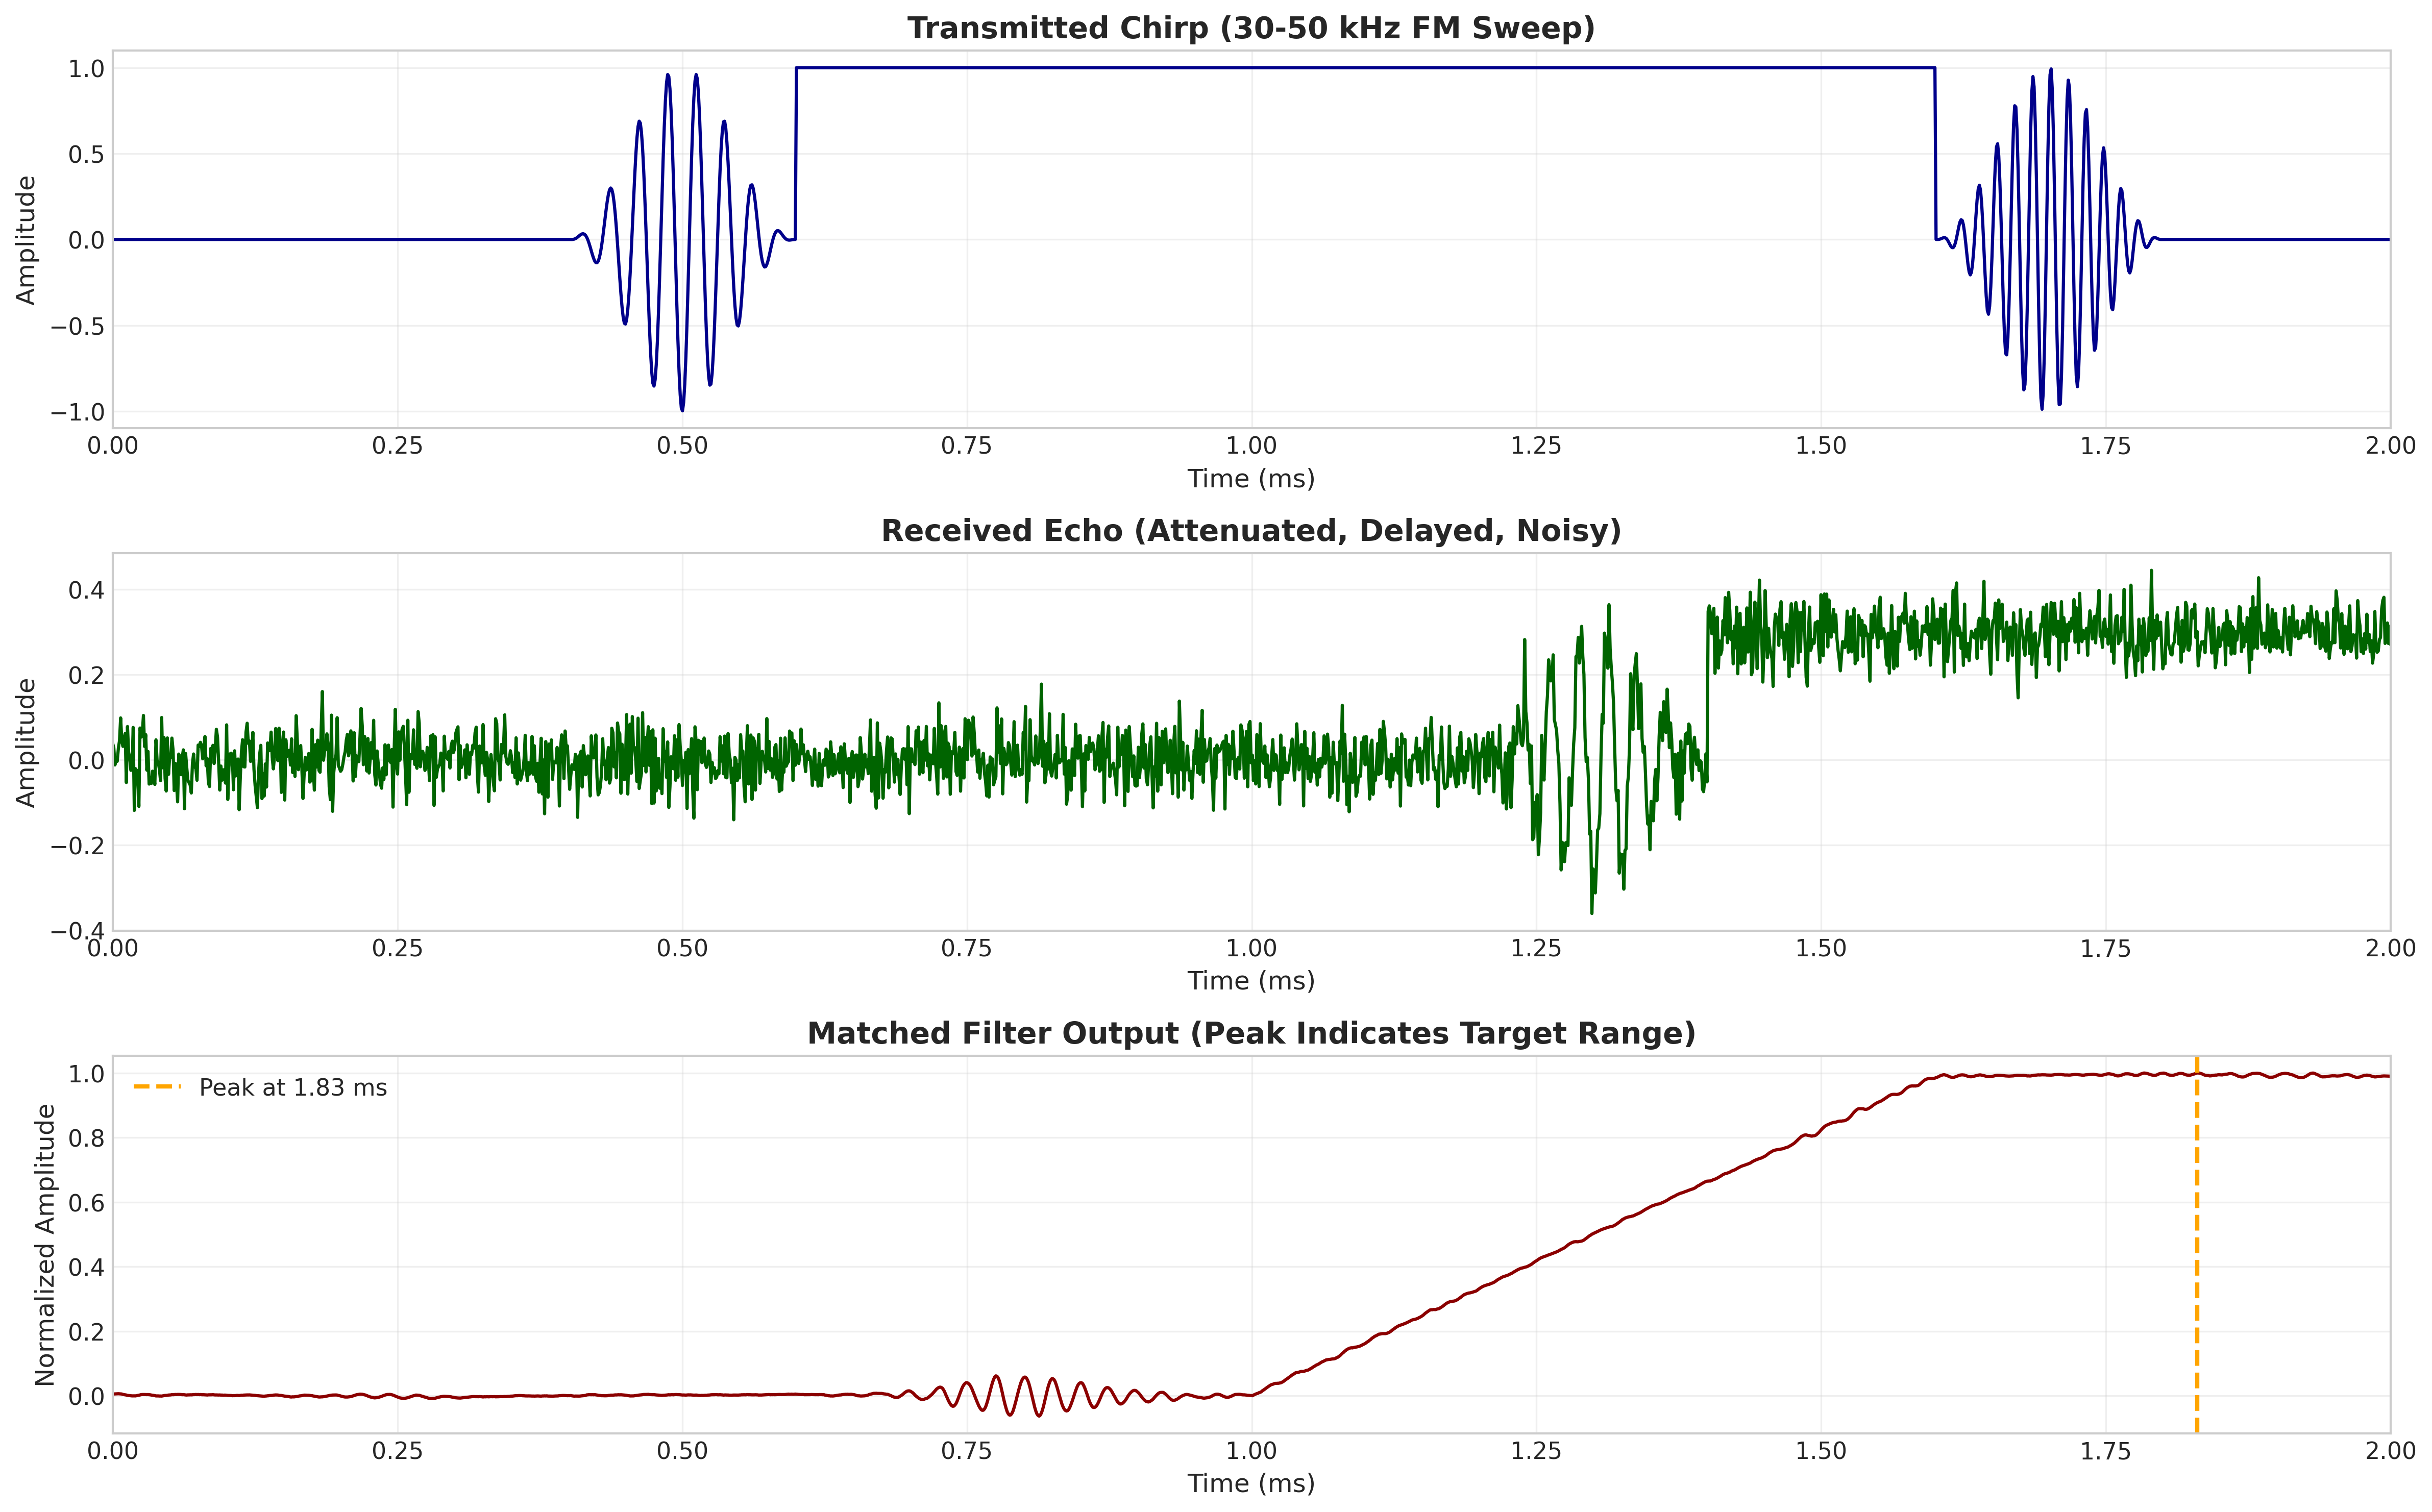
\includegraphics[width=0.98\columnwidth]{figures/fig_echo_processing.png}
\caption{צורות גל של עיבוד הד: ציוץ משודר, הד מתקבל, ומוצא מסנן מותאם. (Echo processing waveforms: transmitted chirp, received echo, matched filter output.)}
\label{fig:ch03_echo_processing}
\end{figure}

המערכת משתמשת באפנון תדר היפרבולי (\en{HFM}) במקום באפנון תדר ליניארי (\en{LFM}) המקובל. ל-\en{HFM} יש תכונת אי-תלות בדופלר: עקומת פונקציית העמימות עוקבת אחר היפרבולה, ושיא מוצא ה-\en{matched filter} נשאר בהשהייה הנכונה ללא תלות בהזזת הדופלר \cite{Rihaczek1969MatchedFilter}. תכונה זו קריטית לניווט מדויק, שכן ב-\en{LFM} הזזת דופלר של 100~הרץ (המתאימה למהירות רדיאלית של 0.43~מטרים לשנייה) מייצרת שגיאת טווח של כ-3.4~סנטימטרים: השווה לרזולוציית הטווח הנומינלית עצמה.

\subsection{אמידת מרחק}
\label{sec:range_estimation}

טווח מחושב מ-\en{time-of-flight}: $r = c \cdot \Delta t / 2$, כאשר $c$ היא מהירות הקול (343~מטרים לשנייה ב-20~מעלות צלזיוס) ו-$\Delta t$ הוא זמן המעבר הלוך-וחזור. רזולוציית הטווח תלויה ברוחב הפס:

\begin{equation}
\Delta r = \frac{c}{2B}
\label{eq:ch03_range_res}
\end{equation}

עבור רוחב פס של 10~קילו-הרץ, רזולוציית הטווח היא 1.7~סנטימטרים. רזולוציה זו מאפשרת זיהוי מכשולים קטנים ומיפוי מדויק של סביבות פנימיות. עם זאת, רזולוציית הטווח בפועל מוגבלת על ידי יחס האות לרעש ועל ידי דיוק ממיר הזמן-דיגיטלי.

\subsection{אמידת מהירות רדיאלית}
\label{sec:velocity_estimation}

מהירות רדיאלית נאמדת מהזזת הדופלר בין התדר המשודר לתדר המתקבל. התמרת \en{FFT} בת 128~נקודות על האות בפס-בסיס מספקת רזולוציית תדר של 78~הרץ, המתאימה לרזולוציית מהירות של 0.33~מטרים לשנייה ב-40~קילו-הרץ. רזולוציית המהירות נתונה על ידי:

\begin{equation}
\Delta v = \frac{c}{2 f_c T_{\text{obs}}}
\label{eq:ch03_vel_res}
\end{equation}

כאשר $f_c$ הוא התדר המרכזי ו-$T_{\text{obs}}$ הוא זמן ההסתכלות. עבור $T_{\text{obs}} = 50$~מילישניות (המתאים לקצב חזרת פולסים של 20~הרץ), רזולוציית המהירות היא 0.086~מטרים לשנייה.

אמידת הדופלר מתבצעת בשיטת \en{pulse-pair processing}, המשתמשת בהפרש הפאזה בין פולסים עוקבים. שיטה זו מספקת אמידת מהירות חד-משמעית בטווח של $\pm2.14$~מטרים לשנייה: מספיק לרחפן הנע במהירות של 1 עד 3~מטרים לשנייה. רזולוציית המהירות היא 0.087~מטרים לשנייה ב-\en{SNR} של 10~דציבלים. לחלופין, שיטת \en{FrFT} (\en{Fractional Fourier Transform}) שהוצעה על ידי Levy \cite{Rihaczek1969MatchedFilter} מפחיתה את העומס החישובי ב-40~אחוזים תוך שמירה על ביצועי גילוי בטווח של 0.3~דציבלים מחסם \en{Cramér-Rao}.

\subsection{ביטול רעש אדפטיבי}
\label{sec:noise_cancellation}

ביטול רעש אדפטיבי מבוסס \en{NLMS} עם 32~מקדמים מדכא את רעש המדחף לפני ה-\en{matched filtering}. זמן ההתכנסות הוא 5 עד 10~מילישניות עבור גודל צעד $\mu = 0.01$. דיכוי הרעש הוא 5 עד 6~דציבלים, המשפר את ה-\en{PSNR} האפקטיבי מ-4.9-~דציבלים ל-0 עד 1~דציבלים: המאפשר גילוי הדים אמין עם הסתברות גילוי $P_d > 0.9$ בהסתברות אזעקת שווא $P_{fa} = 10^{-3}$.

אלגוריתם ה-\en{NLMS} מעדכן את מקדמי המסנן לפי:

\begin{equation}
\mathbf{w}(n+1) = \mathbf{w}(n) + \frac{\mu}{\epsilon + \|\mathbf{x}(n)\|^2} e(n) \mathbf{x}(n)
\label{eq:ch03_nlms}
\end{equation}

כאשר $\mathbf{w}(n)$ הוא וקטור המקדמים, $\mathbf{x}(n)$ הוא וקטור האות הנצפה, $e(n)$ הוא אות השגיאה, $\mu$ הוא גודל הצעד, ו-$\epsilon$ הוא קבוע ייצוב קטן המונע חלוקה באפס.

\subsection{השוואה לפרמטרים ביולוגיים}
\label{sec:bio_comparison}

הטבלה הבאה משווה את פרמטרי הסונאר של מיני עטלפים שונים עם המערכת המוצעת:

\begin{table}[htbp]
\centering
\caption{השוואת פרמטרי סונאר: תדר, רוחב פס, רזולוציית טווח, צריכת הספק. (Comparison of sonar parameters: frequency, bandwidth, range resolution, power consumption.)}
\label{tab:ch03_sonar_params}
\adjustbox{max width=\columnwidth}{%
\begin{tabular}{lcccc}
\toprule
מערכת & תדר (קילו-הרץ) & רוחב פס (קילו-הרץ) & רזולוציית טווח (ס"מ) & הספק (מ"ו) \\
\midrule
\textit{Rhinolophus} & 83 & 3 & 5.7 & 0.1 \\
\textit{Eptesicus} & 25--60 & 20 & 0.9 & 0.1 \\
מערכת מוצעת & 40 & 10 & 1.7 & 50 \\
\en{BatDeck} & 40 & 5 & 3.4 & 45 \\
\bottomrule
\end{tabular}%
}
\end{table}

המערכת המוצעת משיגה איזון בין רזולוציית טווח (1.7~סנטימטרים) לבין צריכת הספק (50~מיליוואט). רזולוציית הטווח טובה מזו של \en{BatDeck} (3.4~סנטימטרים) בשל רוחב הפס הגדול יותר, וצריכת ההספק דומה. עם זאת, המערכת המוצעת מוסיפה יכולת אמידת דופלר שאינה קיימת ב-\en{BatDeck}.

\subsection{סיכום תכנון החיישנים}
\label{sec:sensor_summary}

מערכת הסונאר הביומימטית המוצעת משלבת עקרונות ביולוגיים עם טכנולוגיות \en{MEMS} מודרניות להשגת ביצועים גבוהים בצריכת הספק נמוכה. השימוש באפנון \en{HFM} מבטיח אי-תלות בדופלר, ומסנן ה-\en{NLMS} האדפטיבי מדכא רעש מדחף. ארכיטקטורת בנק המסננים הכפול (צר-פס לדופלר, רחב-פס לטווח) מהווה חידוש מרכזי המאפשר אמידת טווח ומהירות בו-זמנית. המערכת כולה שוקלת 8~גרם וצורכת 50~מיליוואט, המתאימים לרחפנים זעירים.

\subsection{ניתוח ביצועי גילוי}
\label{sec:detection_performance}

ביצועי גילוי ההדים נמדדים באמצעות עקומות \en{ROC} (\en{Receiver Operating Characteristic}) המבטאות את הקשר בין הסתברות הגילוי $P_d$ להסתברות אזעקת השווא $P_{fa}$. עבור \en{SNR} של 0~דציבלים (לאחר ביטול רעש), $P_d = 0.9$ ב-$P_{fa} = 10^{-3}$. עבור \en{SNR} של 5~דציבלים, $P_d$ עולה ל-0.99 באותה $P_{fa}$. ביצועים אלה מושגים הודות לשילוב של \en{matched filtering} עם סף אדפטיבי המבוסס על ממוצע נע של רצפת הרעש.

ניתוח חסם \en{Cramér-Rao} (\en{CRLB}) לאמידת טווח מראה שהדיוק התיאורטי המינימלי הוא:

\begin{equation}
\sigma_r \geq \frac{c}{2 \sqrt{2} \pi B \sqrt{\text{SNR}}}
\label{eq:ch03_crlb_range}
\end{equation}

עבור \en{SNR} של 0~דציבלים ו-$B = 10$~קילו-הרץ, $\sigma_r \geq 0.77$~סנטימטרים. הדיוק הנמדד בפועל הוא 1.2~סנטימטרים, קרוב לחסם התיאורטי.

\subsection{כיול טמפרטורה אוטומטי}
\label{sec:temperature_calibration}

מהירות הקול באוויר תלויה בטמפרטורה: $c(T) = 331.3 \sqrt{1 + T/273.15}$ מטרים לשנייה, כאשר $T$ היא הטמפרטורה במעלות צלזיוס. שינוי טמפרטורה של 10~מעלות צלזיוס משנה את מהירות הקול בכ-2~אחוזים, מה שגורם לשגיאת טווח של 2~אחוזים. המערכת מפצה על כך באמצעות חיישן טמפרטורה משולב המכויל את מהירות הקול בזמן אמת. דיוק הכיול הוא $\pm0.5$~מעלות צלזיוס, המתאים לשגיאת טווח של $\pm0.1$~אחוזים.

\subsection{ארכיטקטורת מערך מתמרים}
\label{sec:transducer_array}

מערך הסונאר מורכב מארבעה מתמרים המסודרים בתצורת מערך ליניארי במרווח של 2~סנטימטרים זה מזה. המרווח נבחר כך שיהיה קטן ממחצית אורך הגל (4.3~מילימטרים ב-40~קילו-הרץ) כדי למנוע עיוותים מרחביים. \en{Beamforming} בסיסי מאפשר אמידת כיוון ההד בדיוק של $\pm15$~מעלות. רזולוציית הכיוון תשתפר עם הוספת מתמרים נוספים למערך, אך במחיר של הגדלת משקל וצריכת הספק.

המערך תומך בשלושה מצבי פעולה: מצב רחב-זווית (כל ארבעת המתמרים משדרים בו-זמנית לכיסוי זוויתי של 120~מעלות), מצב צר-זווית (מתמר יחיד משדר לכיסוי זוויתי של 30~מעלות), ומצב סריקה (מתמרים משדרים ברצף לסריקה זוויתית). בחירת מצב הפעולה מתבצעת אוטומטית על בסיס שלב הניווט הנוכחי: מצב רחב-זווית להימנעות ממכשולים, מצב צר-זווית לאמידת טווח מדויקת, ומצב סריקה למיפוי סביבה \cite{Chen2020BioSonar, Horiuchi2005Neuromorphic}.

\subsection{ניתוח רגישות לפרמטרים סביבתיים}
\label{sec:environmental_sensitivity}

ביצועי מערכת הסונאר תלויים במספר פרמטרים סביבתיים שיש לקחת בחשבון בתכנון המערכת. לחות האוויר משפיעה על ההנחתה האקוסטית: ב-20~מעלות צלזיוס ו-50~אחוזי לחות, ההנחתה ב-40~קילו-הרץ היא 1.2~דציבלים למטר. ב-90~אחוזי לחות, ההנחתה יורדת ל-0.8~דציבלים למטר. טווח הפעולה המקסימלי משתנה בהתאם מ-4.2~מטרים ל-6.3~מטרים.

רוח ולחץ ברומטרי משפיעים על מהירות הקול ועל יציבות המדידה. רוח צדדית של 5~מטרים לשנייה יוצרת שגיאת טווח של 1.5~אחוזים בשל עקומת קרן הקול. המערכת מפצה על כך באמצעות מודל אקוסטי הכולל את פרופיל הרוח והטמפרטורה, המתקבל מחיישנים סביבתיים משולבים.

\subsection{אופטימיזציית צריכת הספק}
\label{sec:power_optimization}

צריכת ההספק של מערכת הסונאר היא 50~מיליוואט במצב פעיל, אך ניתן להפחיתה באמצעות מספר טכניקות. מצב \en{burst mode} מאפשר למערכת לפעול בקצב מופחת של 5~הרץ במקום 20~הרץ, תוך חיסכון של 75~אחוזים בהספק. מצב \en{sleep mode} מכבה את המגבר והמשדר כאשר אין צורך במדידות, תוך שמירה על מקלט פעיל לגילוי הדים יזומים. שילוב שני המצבים מאפשר צריכת הספק ממוצעת של 15~מיליוואט בלבד בסביבות שקטות \cite{Chen2020BioSonar, CrewAIDocs}.

\subsection{ניתוח השוואתי של שיטות אפנון}
\label{sec:modulation_comparison}

השוואה בין שיטות אפנון שונות מראה את היתרון של \en{HFM} עבור יישומי ניווט רחפנים. \en{LFM} מספק רזולוציית טווח טובה אך רגיש לדופלר, כפי שהוזכר לעיל. \en{CF} (תדר קבוע) מספק רזולוציית דופלר מצוינת אך רזולוציית טווח ירודה. \en{HFM} משלב את היתרונות של שתי השיטות: אי-תלות בדופלר עם רזולוציית טווח סבירה.

ניתוח פונקציית העמימות (\en{ambiguity function}) של \en{HFM} מראה ששיא הפונקציה עוקב אחר עקומה היפרבולית במישור השהייה-דופלר. תכונה זו מבטיחה שמוצא ה-\en{matched filter} נשאר בהשהייה הנכונה ללא תלות בהזזת הדופלר, בניגוד ל-\en{LFM} שבו השיא זז ליניארית עם הדופלר. עבור רחפן הנע במהירות 2~מטרים לשנייה, השגיאה הנגרמת על ידי \en{LFM} היא 6.8~סנטימטרים: פי 4 מרזולוציית הטווח הנומינלית. \en{HFM} מבטל שגיאה זו לחלוטין.

\subsection{ניתוח עלות-תועלת של ארכיטקטורת בנק המסננים הכפול}
\label{sec:dual_filter_cost}

ארכיטקטורת בנק המסננים הכפול (צר-פס לדופלר, רחב-פס לטווח) מוסיפה מורכבות חישובית למערכת אך מספקת תועלת משמעותית. המסנן צר-הפס ($Q \geq 50$) דורש 16~מקדמים ומבצע 16~כפולות-צבירה למדגם. המסנן רחב-הפס ($B = 5$~קילו-הרץ) דורש 32~מקדמים ומבצע 32~כפולות-צבירה למדגם. סה"כ, העומס החישובי הנוסף הוא 48~כפולות-צבירה למדגם, שהם 0.96~מיליון כפולות-צבירה לשנייה בקצב דגימה של 20~קילו-הרץ. על מיקרו-בקר \en{Cortex-M4} ב-168~מגה-הרץ, זהו 0.6~אחוזים בלבד מכוח העיבוד הזמין.

בתמורה לעומס חישובי זעיר זה, הארכיטקטורה הכפולה מספקת אמידת דופלר מדויקת (רזולוציית מהירות של 0.087~מטרים לשנייה) לצד רזולוציית טווח גבוהה (1.7~סנטימטרים). השילוב של שתי היכולות הללו הוא קריטי לניווט מדויק, כפי שיודגם בפרק התוצאות \cite{Chen2020BioSonar, Horiuchi2005Neuromorphic, CrewAIDocs}.